% !TEX root = slides.tex

\title{\LaTeX}
\section{\LaTeX}

\begin{frame}[fragile]
  \label{latex}
  \begin{block}{\centering\Large Föreläsning 2 --- \LaTeX}
    Förberedelse inför laboration 2.

    \begin{itemize}
      \ii{Ordbehandling}
      \ii{\LaTeX}
      \ii{Mall för rapport}
      \ii{Dokumentstruktur: dokumentklasser, omgivningar, text, stycken, listor, tabeller, \ldots}
      \ii{Programlistor}
      \ii{Matematiska formler}
      \ii{Bilder}
    \end{itemize}
  \end{block}
\end{frame}


\begin{frame}[fragile]
  \frametitle{Ordbehandling: {\sc Wysiwyg} vs. LaTeX}

  \ti{Två olika sätt att skriva text:}

  \blankline
  \begin{itemize}
    \ii{{\sc Wysiwyg} (What You See Is What You Get)}
    \begin{itemize}
      \ii{Exempel: Microsoft Word}
      \ii{Direkt återspegling av slutresultatet på skärmen}
      \ii{Inkluderar teckensnitt, storlekar, avstånd, etc.}
    \end{itemize}

    \bigskip % Lägger till extra utrymme för tydlighet
    \ii{\LaTeX\ fungerar annorlunda!}
    \begin{itemize}
      \ii{Fokus på innehåll istället för utseende}
      \ii{Skriver kommandon eller ``taggar'' för att uttrycka formatering}
      \ii{Texten \emph{kompileras} till ett formaterat dokument (oftast PDF)}
    \end{itemize}
  \end{itemize}

\end{frame}

\begin{frame}[fragile]
  \frametitle{\LaTeX\ - Arbetssätt och Exempel}


  \ti{I \LaTeX\ skriver man text och formateringskommandon i en textfil.}
  \blankline

  \begin{exlatex}
  För rätvinkliga trianglar gäller \emph{Pythagoras sats}: $a^2 + b^2 = c^2$
  \end{exlatex}

  \blankline
  \ti{Tecknet \code{\$} markerar början och slutet på matematiska uttryck. \LaTeX\ hanterar automatiskt stil och placering för matematiska element.}

\end{frame}



\begin{frame}[fragile]
  \frametitle{Interaktiv Demonstration}

  \begin{center}
    \Huge Demo!

    \bigskip
    \Large Jämför {\sc Wysiwyg} med \LaTeX
  \end{center}

\end{frame}


% \begin{frame}[fragile]
% \frametitle{Layout av text}
% I de flesta ordbehandlare finns det
% formatmallar där man till exempel kan bestämma att alla rubriker på
% en viss nivå ska ha ett visst utseende. Om man vill ändra
% utseendet på alla rubriker så räcker det att ändra i mallen.

% \blankline
% Det brukar också finnas möjlighet till automatisk numrering av 
% rubriker, automatisk generering av innehållsförteckning och 
% sakregister och liknande. 

% \blankline
% När man skriver matematisk text använder man ofta en ekvationseditor
% för att skriva de matematiska symbolerna. Ekvationseditorer är inte
% enkla att använda, och slutresultatet brukar inte bli bra.
% \end{frame} 


\begin{frame}[fragile]
  \frametitle{Ett större exempel}
  \begin{exlatex}
If $f$ is continuous on the closed interval $a \leq x \leq b$ and differentiable on the open interval $a < x < b$, then there exists a point $\xi$, $a < \xi < b$ such that:

\begin{displaymath}
  f(b) - f(a) = f'(\xi)(b - a).
\end{displaymath}
  \end{exlatex}

\end{frame}

\begin{frame}[fragile]
  \frametitle{\LaTeX-historik}
  \begin{itemize}
    \ii{Donald E. Knuth, \TeX\ från 1977}
    \ii{''Tech''—precision i typsättning}
    \ii{Leslie Lamport utvecklar \LaTeX\ på 1980-talet}
    \ii{Förenklar \TeX, fokus på innehåll}
    \ii{Bred användning inom akademi och industri}
  \end{itemize}
  \note{
    \begin{itemize}
      \item \TeX\ skapades av Donald Knuth som svar på bristerna i akademisk textproduktion.
      \item Leslie Lamport byggde vidare på detta och gjorde \TeX\ tillgängligt för en bredare publik genom \LaTeX.
      \item \LaTeX\ tillåter forskare och författare att fokusera på innehållets kvalitet snarare än dess presentation.
      \item Används för vetenskapliga dokument, böcker, och akademiska publikationer.
    \end{itemize}
  }
\end{frame}

\begin{frame}[fragile]
  \frametitle{Arbeta med \LaTeX}
  \begin{itemize}
    \ii{Skrivs i vanliga textfiler, filändelse \code{.tex}}
    \ii{Kompilera till \code{pdf} med kommandot \code{pdflatex}}
    \ii{Specialiserade \LaTeX-verktyg: \code{texmaker}, \code{TeXShop}, \code{TeXstudio}}
    \ii{VS Code med \code{LaTeX Workshop}-tillägg}
    \ii{Finns andra kompilatorer: \code{pdflatex} (vanligast), \code{XeLaTeX} (modernare, UTF-8)}
  \end{itemize}
  \note{
    \begin{itemize}
      \item \code{.tex}-filer är rena textfiler som kan redigeras med vilken textredigerare som helst.
      \item \code{pdflatex} är standardkompilatorn och fungerar bra för de flesta dokument.
      \item Integrerade verktyg som \code{texmaker}, \code{TeXShop}, och \code{TeXstudio} erbjuder enklare gränssnitt för att redigera, kompilera och visa \LaTeX-dokument.
      \item \code{VS Code} är en populär editor för många programmeringsspråk, och med \code{LaTeX Workshop}-tillägget blir den ett kraftfullt verktyg för \LaTeX.
      \item \code{XeLaTeX} erbjuder bättre stöd för moderna typografiska funktioner och fullt stöd för Unicode, vilket gör den idealisk för dokument som inkluderar flera språk eller specialtecken.
    \end{itemize}
  }
\end{frame}


\begin{frame}
  \frametitle{Fördelar med \LaTeX}
  \begin{itemize}
    \ii{Professionellt utseende}
    \ii{Automatisk numrering av rubriker, figurer, tabeller}
    \ii{\textbf{Källkoden är ren text} -- Varför är det bra? :) }
    \ii{Lätt att skapa och referera till tabeller, figurer, ekvationer}
    \ii{Automatisk innehållsförteckning}
    \ii{Bra stöd för matematiska formler}
    \ii{Gratis och plattformsoberoende, fungerar på Windows, MacOS, Linux}
    \ii{Omfattande community och resurser -- kan dock vara överväldigande och ibland stöter man på obskyra problem}
  \end{itemize}
  \note{
    \begin{itemize}
      \item \LaTeX ger dokument ett professionellt och konsekvent utseende automatiskt.
      \item Ren text-format gör det lätt att använda verktyg som Git för versionskontroll, vilket är idealiskt för samarbetsprojekt.
      \item \LaTeX-communityt erbjuder omfattande stöd och resurser, vilket gör det lätt att få hjälp och lära sig mer om avancerade funktioner.
      \item Varning för att det stora antalet paket och funktioner ibland kan kännas överväldigande och leda till att man stöter på mindre vanliga problem.
    \end{itemize}
  }
\end{frame}


\begin{frame}
  \frametitle{Dags att hoppa in i \LaTeX!}

  % "Paus"-slide innan vi går vidare till detaljer
  \begin{center}
    \Huge Nu dyker vi ner i detaljerna!
  \end{center}
\end{frame}

\begin{frame}[fragile,t]
  \frametitle{Dokumentklasser}
  \vspace{3em}
  \begin{itemize}
    \ii{\emph{Dokumentklassen} styr dokumentets övergripande utseende.}
    \ii{Vanliga dokumentklasser: \code{article}, \code{report}, \code{book}, \code{letter}, \code{beamer}.}
    \ii{\code{article} används mest; \code{beamer} för presentationer.}
  \end{itemize}

  \blankline
  \begin{envi}
    \begin{lstlisting}[style=latexex]
      % Exempel på användning av dokumentklassen article
      \documentclass{article}
      \begin{document}
      Hej världen! Detta är ett enkelt dokument.
      \end{document}
    \end{lstlisting}
  \end{envi}

  \note{
    \begin{itemize}
      \item \code{article} är idealisk för vetenskapliga artiklar, rapporter och anteckningar.
      \item \code{beamer} används för att skapa visuellt engagerande presentationer.
    \end{itemize}
  }
\end{frame}

\begin{frame}[fragile,t]
  \frametitle{Använda Kommandon i LaTeX}

  \begin{itemize}
    \ii{\LaTeX-kommandon styr hur text formateras och struktureras.}
    \ii{Kan ändra typsnitt, storlek, färg, och mer.}
    \ii{De kan även organisera text i avsnitt, listor och tabeller.}
  \end{itemize}

  \begin{exlatex}
% Ex: enkelt kommando
\textbf{Fetstil} gör texten fet, \textit{kursiv stil} gör texten kursiv. Ofta används \emph{emfas} för att markera \emph{viktig text}.

% Ex: listor enumerate/itemize
\begin{enumerate}
  \item Listor hjälper till att organisera information.
  \item Varje \item skapar en ny punkt i listan.
\end{enumerate}
  \end{exlatex}
  
  \note{
    Kommandon i LaTeX skrivs med en backslash (\textbackslash) och kan ha parametrar både före och efter texten som de formaterar.
    - T.ex., \textbackslash textbf\{text\} applicerar fetstil.
    - Komplexa kommandon som \textbackslash begin\{itemize\} används för att skapa strukturerade format som listor.
  }

\end{frame}

\begin{frame}[fragile,t]
  \frametitle{Omgivningar}
  \vspace{1em}
  \begin{itemize}
    \ii{Kommandon som innehåller flera rader text kallas \emph{omgivningar}.}
    \ii{En omgivning definieras av \code{\textbackslash begin\{...\}} och \code{\textbackslash end\{...\}}.}
    \ii{Omgivningar påverkar utseendet för det innehåll de omsluter.}
  \end{itemize}

  \blankline
  \begin{envi}
    \begin{exlatex}
% Exempel på en enkel omgivning
\begin{itemize}
  \item Detta är en punktlista.
  \item Listor hjälper till att organisera information.
  \item Denna punkt har flera delar
  \begin{enumerate}
    \item Första delen
    \item Och resten
  \end{enumerate}
\end{itemize}
    \end{exlatex}
  \end{envi}

  \note{
    \begin{itemize}
      \item \code{itemize} omgivningen är bra för att skapa punktlistor.
      \item Varje \code{item} representerar en punkt i listan..
    \end{itemize}
  }
\end{frame}



% \begin{frame}[fragile]
%   \frametitle{Löpande text}
%   Radslut och antal mellanslag mellan ord har ingen betydelse,
%   \LaTeX\ formaterar så att det blir snyggt. En
%   eller flera blanka rader ger ett nytt stycke. Exempel:

%   \bex
%   Det här
%   är en text som jag
%   har    skrivit. Det är
%   en lång text med flera
%   rader.

%   Här börjar det ett
%   nytt stycke i texten.
%   \end{verbatim}
%   \mex
%   Det här
%   är en text som jag
%   har    skrivit. Det är
%   en lång text med flera
%   rader.

%   \hspace{1em}Här börjar det ett
%   nytt stycke i texten.
%   \eex
% \end{frame}

% \begin{frame}[fragile]
%   \frametitle{Rubriker}
%   \LaTeX\ numrerar rubriker automatiskt. Man anger en rubrik med
%   \verb+\section+ eller \verb+\subsection+.

%   \bex
%   \section{Inledning}
%   \section{Utförande}
%   \subsection{Del 1}
%   \subsection{Del 2}
%   \section{Slutsatser}
%   \end{verbatim}
%   \mex
%   {\Large\bfseries 1 Inledning} \\[1ex]
%   {\Large\bfseries 2 Utförande} \\[1ex]
%   {\large\bfseries 2.1 Del 1} \\[1ex]
%   {\large\bfseries 2.2 Del 2} \\[1ex]
%   {\Large\bfseries 3 Slutsatser}
%   \eex

% \end{frame}

% \begin{frame}[fragile]
%   \frametitle{Ändra textens utseende}
%   Det finns många kommandon för att ändra utseende på texten. Två
%   sådana kommandon  är \verb+\emph+ för att betona text och \verb+\texttt+
%   för att skriva med skrivmaskinstypsnitt. Exempel:

%   \begin{exempel}
%     Här skriver jag något
%     \emph{viktigt}. Och
%     i Java har vi använt
%     klassen \texttt{Square}.
%   \end{exempel}

%   Det finns också kommandon för fetstil, lutande text, osv, och för att
%   ändra storlek på texten. Använd sparsamt!
% \end{frame}

% \begin{frame}[fragile]
%   \frametitle{Specialtecken}
%   Med tecknet \code{\%} inleder man en kommentar som sträcker sig till slutet av raden.

%   \blankline
%   En del tecken används för kommandon och måste skrivas på speciellt sätt:

%   \begin{Code}
%     \$ \% \_ \# \& \{ \} \textbackslash
%   \end{Code}

%   Det finns streck, mellanrum och punkter av olika slag:

%   \begin{exempel}
%     DoD-kursen pågår under vecka
%     1--3 av läsperiod ht1. Tyvärr
%     är den inte längre \ldots

%     \quad Telefon: 046--222~80~38.
%     Dagens datum: \today.
%   \end{exempel}
% \end{frame}

% \begin{frame}[fragile]
%   \frametitle{Fotnoter}
%   Fotnoter är lätta att skriva:

%   \bex
%   Om man använder \LaTeX
%   \footnote{uttalas
%     ''lah-tekh''} så
%   blir det bra. Alla rapporter
%   blir automatiskt snyggt
%   utformade.
%   \end{verbatim}
%   \mex
%   Om man använder \LaTeX
%   \footnote{uttalas
%     ''lah-tekh''} så
%   blir det bra. Alla rapporter
%   blir automatiskt snyggt
%   utformade.
%   \eex

%   Fotnoter numreras automatiskt 1,2,\ldots
%   Fast här blev ''numret'' på fotnoten ''a'' av olika anledningar.
%   Observera att man skriver två apostrofer (\verb+''+) i stället
%   för citationstecken (\code{"}).
% \end{frame}

% \begin{frame}[fragile]
%   \frametitle{Listor}
%   Punktlistor är enkla:

%   \begin{exempel}
%     \begin{itemize}
%       \ii{första punkten}
%       \ii{här kommer den andra}
%       punkten i listan
%     \end{itemize}
%   \end{exempel}

%   Numrerade listor är lika enkla:

%   \begin{exempel}
%     \begin{enumerate}
%       \ii{första punkten}
%       \ii{här kommer den andra}
%       punkten i listan
%     \end{enumerate}
%   \end{exempel}

%   OBS! Pga hur detta dokument är formaterat så får listelementen inga punkter eller siffror, men i den vanliga dokumentklassen \code{\{article\}} blir det som förväntat.
%   % I detta dokument används dokumentklassen \code{beamer}, och där blir numren siffror i cirklar. I den vanliga dokumentklassen \code{\{article\}} blir numren 1., 2., \ldots
% \end{frame}

% \begin{frame}[fragile]
%   \frametitle{Definitioner}
%   \begin{exempel}
%     Några klasser som vi använder:

%     \begin{description}
%       \di{SimpleWindow}{Beskriver ett}
%       enkelt ritfönster
%       \di{Scanner}{Inläsning från}
%       tangentbordet
%       \di{Random}{Slumptal}
%     \end{description}
%   \end{exempel}

%   I dokumentklassen \code{article} blir det något annorlunda layout på definitioner. Använd en \code{tabular}-omgivning med kolumnspecifikationen \code{p\{bredd\}} för att få layout som liknar den ovan.
% \end{frame}

% \begin{frame}[fragile]
%   \frametitle{Tabeller}
%   En tabell där den första kolumnen är vänsterinpassad (\code{l}), den
%   andra centrerad (\code{c}) och den tredje högerinpassad (\code{r}). \code{\&} avgränsar kolumnerna,
%   \verb+\\+ betyder ny rad, \verb+~+ är ett ''hårt'' blanktecken. \verb+\hline+ är ett streck.

%   \bex
%   \begin{tabular}{lcr}
%     Produkt & Typ    & Pris    \\
%     \hline
%     Skruvar & stora  & 0.18~kr \\
%     Muttrar & M16    & 0.38~kr \\
%     Spikar  & 12~tum & 0.12~kr
%   \end{tabular}
%   \end{verbatim}
%   \mex
%   \begin{tabular}[t]{lcr}
%     Produkt & Typ    & Pris    \\
%     \hline
%     Skruvar & stora  & 0.18~kr \\
%     Muttrar & M16    & 0.38~kr \\
%     Spikar  & 12~tum & 0.12~kr
%   \end{tabular}
%   \eex
% \end{frame}

% \begin{frame}[fragile]
%   \frametitle{Flytande tabeller}
%   Med en \verb+\table+-omgivning skapar man en tabell med en förklarande
%   text och ett nummer. \LaTeX\ placerar tabellen där det är
%   lämpligt.

%   \bex
%   \begin{table}
%     \begin{tabular}{lcr}
%       Produkt & Typ    & Pris    \\
%       \hline
%       Skruvar & stora  & 0.18~kr \\
%       Muttrar & M16    & 0.38~kr \\
%       Spikar  & 12~tum & 0.12~kr
%     \end{tabular}
%     \caption{Våra produkter}
%   \end{table}
%   \end{verbatim}
%   \mex
%   \begin{tabular}[t]{lcr}
%     Produkt & Typ    & Pris    \\
%     \hline
%     Skruvar & stora  & 0.18~kr \\
%     Muttrar & M16    & 0.38~kr \\
%     Spikar  & 12~tum & 0.12~kr
%   \end{tabular}
%   \begin{center}
%     {Tabell 7. Våra produkter}
%   \end{center}
%   \eex
% \end{frame}

% \begin{frame}[fragile]
%   \frametitle{Att referera till etiketter}
%   Om man sätter en etikett på en tabell kan man referera till den
%   från texten. Exempel:

%   \bex
%   \begin{table}
%     \begin{tabular}{lcr}
%       Produkt & Typ   & Pris    \\
%       \hline
%       Skruvar & stora & 0.18~kr \\
%     \end{tabular}
%     \caption{Våra produkter}
%     \label{produkter}
%   \end{table}
%   Senare i texten: våra produkter
%   finns i tabell~\ref{produkter}.
%   \end{verbatim}
%   \mex
%   \begin{tabular}[t]{lcr}
%     Produkt & Typ   & Pris    \\
%     \hline
%     Skruvar & stora & 0.18 kr \\
%   \end{tabular}
%   \begin{center}
%     {Tabell 7. Våra produkter}
%   \end{center}
%   Senare i texten: våra produkter
%   finns i tabell~7.
%   \eex
%   Figurer hanteras likadant som tabeller, i en
%   \verb+\figure+-omgivning.
% \end{frame}

% \begin{frame}[fragile]
%   \frametitle{Programlistor}
%   För att infoga en programlista i en rapport använder man
%   kommandot \verb+\VerbatimInput{filnamn}+ från paketet
%   \texttt{fancyvrb}. Man bör \emph{inte} använda ''standard''-
%   kommandot \verb+\verbatiminput+ eftersom det kommandot
%   ignorerar alla tabulatortecken i programmet, och det medför att
%   indragningarna försvinner.

%   \bex
%   \usepackage{fancyvrb}
%   \fvset{tabsize=4}
%   \fvset{fontsize=\small}

%   \VerbatimInput{Point.java}
%   \end{verbatim}
%   \mex
%   %\vspace{-30pt}
%   \begin{verbatim}
% class Point {
%     private int x;
%     private int y;

%     public Point(int x, int y) {
%         this.x = x;
%         this.y = y;
%     }
% }
% \end{verbatim}
%   \eex
% \end{frame}

% \begin{frame}[fragile]
%   \frametitle{Öka eller minska avstånd}
%   Ibland behöver man öka avståndet i vertikalled mellan två avsnitt i texten, till exempel före eller efter en tabell. Det kan man göra med kommandot \verb/\vspace{längd}/, där längden kan anges i millimeter eller punkter eller något annat som \LaTeX\ känner igen. Längden kan vara negativ om man vill minska avståndet. Det finns också specialkommandon för att lägga in ett litet, mellanstort och stort avstånd:

%   \begin{Code}
%     \smallskip  \medskip  \bigskip
%   \end{Code}

%   Man kan öka eller minska horisontellt avstånd med \verb/\hspace{längd}/.
% \end{frame}

% \begin{frame}[fragile]
%   \frametitle{Matematiska formler}
%   \LaTeX\ är \emph{mycket} bra på att formatera matematisk text.
%   Alla (tror jag) artiklar och böcker som innehåller matematiska formler
%   är skrivna med \LaTeX. Man kan skriva
%   formler antingen inuti löpande text eller på en egen rad:
%   \begin{itemize}
%     \ii{I texten: formeln inleds med \code{\$} och avslutas med \code{\$}.}
%     \item<+-> På egen rad: formeln inleds med \verb+\begin{displaymath}+
%           och avslutas med \verb+\end{displaymath}+.
%           \verb+\begin{equation}+ och \verb+\end{equation}+ ger samma
%           resultat men formeln numreras. Med \verb+\label+ och \verb+\ref+
%           kan man etikettera och referera till ekvationer.
%   \end{itemize}
% \end{frame}

% \begin{frame}[fragile]
%   \frametitle{Enkla formler}
%   \begin{mexempel}
%     Formeln $x=3y-2$ står
%     inne i texten. Däremot
%     står
%     \begin{displaymath}
%       x=3y-2
%     \end{displaymath}
%     för sig själv precis som
%     \begin{equation}
%       x=3y-2
%       \label{xochy}
%     \end{equation}
%     I ekvation~\ref{xochy} fann
%     vi att \ldots
%   \end{mexempel}
% \end{frame}

% \begin{frame}[fragile]
%   \frametitle{Symboler, index}
%   \begin{mexempel}
%     \begin{displaymath}
%       \alpha \leq \pi \approx 3.141592654
%     \end{displaymath}
%   \end{mexempel}

%   \vspace{1cm}

%   \begin{mexempel}
%     \begin{displaymath}
%       x_{k+1}=x_{k}-f(x_{k})/f'(x_{k})
%     \end{displaymath}
%   \end{mexempel}
% \end{frame}

% \begin{frame}[fragile]
%   \frametitle{Exponenter, rötter}
%   \begin{mexempel}
%     \begin{displaymath}
%       e^x = 1+x+x^2/2!+x^3/3!+\cdots
%     \end{displaymath}
%   \end{mexempel}

%   \vspace{1cm}

%   \begin{mexempel}
%     \begin{displaymath}
%       x_{1,2}=\frac{p}{2}\pm
%       \sqrt{\frac{p^2}{4}-q}
%     \end{displaymath}
%   \end{mexempel}

% \end{frame}



% \begin{frame}[fragile]
%   \frametitle{Integraler, summor}
%   \begin{mexempel}
%     \begin{displaymath}
%       \int_{-\infty}^{\infty}
%       e^{-x^2} dx
%     \end{displaymath}
%   \end{mexempel}

%   \vspace{1cm}

%   \begin{mexempel}
%     \begin{displaymath}
%       \sum_{k=1}^n\frac{1}{a_k}
%     \end{displaymath}
%   \end{mexempel}

% \end{frame}

% \begin{frame}[fragile]
%   \frametitle{Funktioner}
%   \begin{mexempel}
%     \begin{displaymath}
%       \sin^2 x + \cos^2 x = 1
%     \end{displaymath}
%   \end{mexempel}
% \end{frame}

% \begin{frame}[fragile]
%   \frametitle{Matriser, parenteser}
%   \begin{mexempel}
%     \begin{displaymath}
%       A=\left(
%       \begin{array}{cccc}
%         a_{11} & a_{12} & \cdots & a_{1n} \\
%         a_{21} & a_{22} & \cdots & a_{2n} \\
%         \vdots & \vdots & \ddots & \vdots \\
%         a_{n1} & a_{n2} & \cdots & a_{nn} \\
%       \end{array}
%       \right)
%     \end{displaymath}
%   \end{mexempel}
% \end{frame}

% \begin{frame}[fragile]
%   \frametitle{Bilder}
%   Bilder kan inkluderas i \LaTeX-dokument om de är i formatet
%   \code{pdf}, \code{jpeg} eller \code{png} (\texttt{eps} om man använder \code{latex}). Man måste använda paketet \texttt{graphicx} (eller \code{graphics}).
%   \vspace{20mm}
%   \bex
%   \usepackage{graphicx}

%   
\includegraphics[height=40mm]{images/bild.pdf}
%   \end{verbatim}
%   \mex
%   \vspace{-25mm}\hspace{15mm}
%   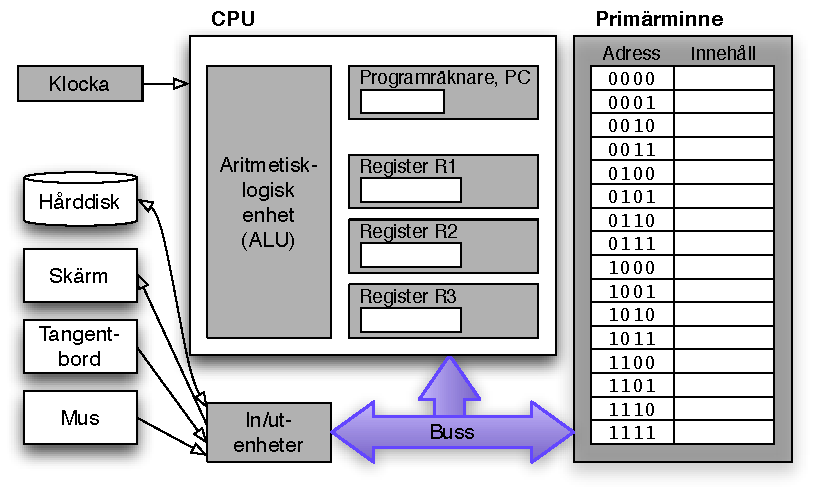
\includegraphics[height=30mm]{images/enkelmodell.pdf}
%   \eex

%   ImageMagick-programmet \texttt{convert} kan konvertera
%   från och till de flesta bildformat:
%   \begin{verbatim}
%    convert bild.fig bild.pdf
% \end{verbatim}
% \end{frame}

% \begin{frame}[fragile]
%   \frametitle{Egna kommandon}
%   Man kan lätt definiera egna kommandon, till exempel ett kortare namn
%   för en text som man använder ofta. Kommandon kan ha parametrar.

%   \vspace{10mm}

%   \begin{mexempel}
%     \newcommand{\java}[1]
%     {\texttt{#1}}

%     Klasser: \java{Random},
%     \java{Scanner} och
%     \java{PrintStream}.
%   \end{mexempel}

%   \vspace{10mm}

%   Man kan definiera om existerande kommandon med
%   \verb+\renewcommand+. Det kan ställa till förvirring, så
%   gör inte det.
% \end{frame}

%\begin{frame}[fragile]
%\frametitle{\LaTeX\ på egen dator}
%
%En sammanfattning av LaTeX-installationer finns på \url{www.latex-project.org}, sidan Getting LaTeX.
%
%\begin{description}
%\item[Linux] LaTeX kanske redan finns på datorn; hämtas annars med den vanliga pakethanteraren.
%\item[Mac] Använd MacTeX (bygger på TeXLive, som uppdateras varje år).
%\item[Windows] proTeXt verkar vara enklast.
%\end{description}
%
%Som IDE rekommenderas Texmaker (\url{www.xm1math.net/texmaker}) eller TeXShop (bara för Mac, \url{www.texshop.org}).
%\end{frame} 

